\subsection{Création du moteur de jeu 3D}
    Pour composer les éléments du jeu et assurer une bonne qualité
    graphique et technique, le choix d'assembler le \emph{moteur de jeu 3D}
    \og \emph{RaptiquaX} \fg{} a été convenu. \emph{\Gls{SDL2}} permet un affichage dans un contexte
    \emph{\Gls{openGL}}, la librairie graphique la plus utilisée dans
    l'industrie du jeu vidéo avec la librairie \emph{Vulkan}
    \footnote{Vulkan \small{(anciennement \emph{OpenGL Next})}, a été
    développé par le groupe Khronos comme le successeur qui remplacera
    \Gls{openGL}.}.

    Pour permettre une composition modulable et accessible à tous, le modèle
    d'architecture de \emph{Godot}\footnote{Godot - 2014 - est un moteur de
    jeu libre multiplateforme proposant à la fois une interface en 2\up{e} et
    en 3\up{e} dimension.} a été utilisé comme référence, en raison de son
    potentiel\footnote{Godot a été très utilisé ces dernières années, même
    dans la réalisation de jeu dit AAA comme
    Sonic Colors Ultimate\cite{soniccoloru} }.

\subsubsection{Conception du moteur de rendu (OpenGL)}
    Un moteur de rendu graphique moderne sous \emph{\Gls{GLSL}} (ou ses
    alternatives\footnote{p. ex. HLSL sous Direct3D}) permet deux pipelines
    différentes et incompatibles\footnote{Depuis quelques années, la pipeline
    "Forward+" cherchant à mêler les deux par des méthodes avancées s'est
    popularisé.} \cite{iehl_deferred_vs_forward} :\\
    \begin{itemize}
        \item Le rendu différé qui permet d'appliquer le \gls{fragment shader}
        une seule fois par \gls{fragment} en utilisant plusieurs couches de
        rendu.
        \item Le rendu direct qui affiche immédiatement sans précalculer le
        \gls{GBuffer} ce qui peut s'avérer plus rapide selon le
        contexte.\\
    \end{itemize}

    Nous avons opté pour l'utilisation du rendu différé, car il permet de
    gérer plus facilement les effets de post-processing et d'optimiser le
    rendu de la lumière. De plus, il est plus adapté pour les scènes
    complexes avec de nombreux objets et lumières. (Pour aller plus loin sur
    le sujet, voir la section \ref{sec:deferred_rendering}).


    Le traitement de l'image est effectué majoritairement par le \gls{gpu},
    exploitant la stratégie inventée pas Silicon Graphics\cite{silicon_graphics}
    pour le traitement de l'image :\\
    \begin{itemize}
        \item Le \Gls{gpu} est divisé en plusieurs unités de calcul
        \item Chaque unité de calcul est responsable d'un aspect du rendu
        \item Les unités de calcul travaillent en parallèle pour traiter
        l'image rapidement
        \item La géométrie est transformée en primitives (triangles, lignes, points) par un programme appelé \emph{\gls{vertex shader}} (figure \ref{fig:sm64_wireframe})
        \item Les primitives sont ensuite \glslink{rasteriser}{rasterisées} pour créer des \glspl{fragment} (figure \ref{fig:sm64_result})\\
    \end{itemize}

    \begin{figure}[h]
        \begin{subfigure}{0.5\textwidth}
            \centering
            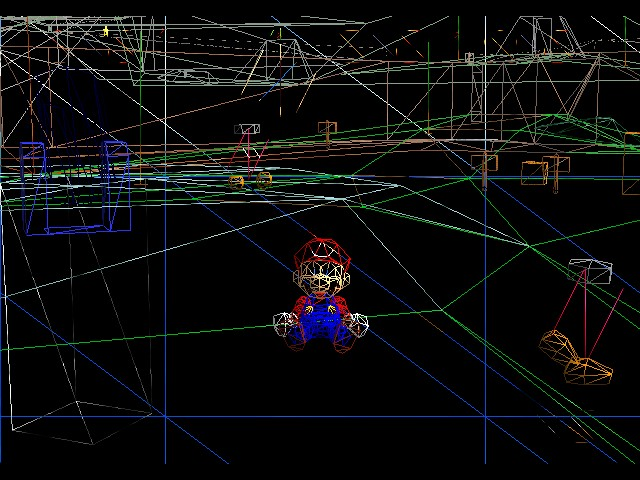
\includegraphics[width=0.8\textwidth]{images/m64wireframe.jpg}
            \caption{Super Mario 64 en mode fil de fer pour imager le \gls{vertex shader}}
            \label{fig:sm64_wireframe}
        \end{subfigure}
        \begin{subfigure}{0.5\textwidth}
            \centering
            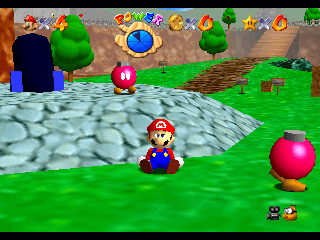
\includegraphics[width=0.8\textwidth]{images/m64result.png}
            \caption{Super Mario 64, après le passage par le \gls{fragment shader}}
            \label{fig:sm64_result}
        \end{subfigure}
        \caption{Exemple de rendu avec la stratégie de Silicon Graphics \cite{copetti_n64}}
        \label{fig:silicon_graphics_rendering}
    \end{figure}

    \newpage
    Enfin, le \gls{gpu} est de nouveau solicité pour le rendu de la scène
    finale, en utilisant les informations de la scène stockées dans le
    \gls{GBuffer} et en appliquant les effets de post-processing.
    Dans notre moteur, nous avons implémenté les techniques de rendu suivantes :
    \begin{itemize}
        \item Le rendu différé
        \item Le rendu de la lumière en suivant le modèle de Phong 
        \item Le rendu des ombres en utilisant le \gls{shadow mapping}
        \item Le rendu de réflexions et de reflets en utilisant le \gls{ssr} (à but expérimental en utilisant le \gls{shader} de \emph{Imanol Fotia} \cite{imanolfotia})
        \item Le rendu d'occlusion ambiante en utilisant le \gls{ssao}
        \item Le rendu d'éblouissement en utilisant le \gls{bloom}
        \item L'anti-aliasing en utilisant le \gls{smaa}
    \end{itemize}

    Une grande partie de ces techniques sont inspirées des travaux de Joey de Vries
    dans son site web LearnOpenGL \cite{learnopengl}, auquels nous avons
    ajouté des améliorations et des optimisations pour notre moteur grâce
    aux travaux de Adrian Courrèges sur DOOM 2016 \cite{courreges_doom2016}.
    \\ \\
    Pour un aperçu de la pipeline graphique de notre moteur, voir la section
    \ref{sec:graphics_pipeline}.

\subsubsection{Conception du moteur de physique}

    Le moteur de physique est responsable de la gestion des collisions et
    des interactions entre les objets de la scène. Il utilise un système de
    détection de collisions basé sur des formes géométriques simples, comme
    des sphères, des boîtes aux transformations non uniforme, des plans, etc.
    \\ \\
    La physique est ensuite calculée en utilisant une approche simplifiée des
    équations \emph{cinématiques} et des équations du \emph{principe fondamental de la dynamique}
    (\emph{deuxième loi de Newton}).

    \newpage

    Soit deux objets rigides, \( A \) et \( B \), se déplacent et entrent
    en collision. \( A \) et \( B \) se repoussent mutuellement selon les
    forces de contact, qui sont proportionnelles à la vitesse de choc et à la
    masse de chaque objet, tel que décrit par les équations de la section \ref{sec:physics_equations}.

\subsubsection{Conception de l'arbre de données}

    Dans notre moteur, nous avons choisi d'utiliser un arbre de données
    pour représenter la scène 3D. Cet arbre est composé de n\oe{}uds, où
    chaque n\oe{}ud représente un objet de la scène. Chaque n\oe{}ud
    contient des informations sur la position, la rotation et l'échelle de
    l'objet, ainsi que des références vers ses enfants et son père.
    Cela permet de créer une hiérarchie d'objets, où chaque objet peut
    être transformé indépendamment tout en étant affecté par les
    transformations de ses parents.
    \\ \\
    Ce modèle d'arbre de données est inspiré du moteur de jeu Godot, qui
    utilise également un arbre de n\oe{}uds pour représenter une scène.
    \\ \\
    Les n\oe{}uds de l'arbre sont génériques, ce qui garantit un stockage
    efficace des données et une gestion facile des objets de la scène (figure \ref{fig:node_structure}).

    \begin{figure}[h]
        \centering
        \includesvg[width=\linewidth]{images/node.svg}
        \emph{La structure présentée ici est une simplification de la structure utilisée dans notre moteur de jeu.}
        \caption{Structure d'un noeud générique}
        \label{fig:node_structure}
    \end{figure}

    Vous pouvez vous référer à la table \ref{tab:raptiquax_nodes} pour découvrir
    les différents types de n\oe{}uds que nous avons implémentés dans notre
    moteur de jeu. Chaque n\oe{}ud est responsable d'un aspect spécifique de
    la scène, ce qui permet de créer un tout cohérent et fluide.


\subsubsection{Conception des classes et héritage}

    Pour assurer une bonne organisation du code et une gestion efficace
    des objets de la scène, nous avons utilisé un système de classes capable
    de gérer l'héritage.
    \\ \\
    Le code source du moteur est précompilé par un outil développé par nos
    soins, qui permet de générer un code source en C à partir d'un fichier
    classe inspiré de la syntaxe de \emph{C++}. Les classes ainsi générées
    sont ensuites liées entre elles par un header de liaison, lui aussi
    généré par l'outil. Cela permet de créer un code source propre et
    facilement lisible, tout en assurant une bonne gestion de la mémoire et des
    performances.
    \\ \\
    Un exemple des classes utilisées par l'outil de précompilation est
    présenté dans le listing \ref{lst:class_template}.
    \\ \\
    Le code source généré utilise les arguments variadiques et prend en charge
    les promotions automatiques des types.
\subsubsection{Conception des entrées sorties}

    Le moteur prend en charge les entrées/sorties de sorte à permettre
    aux développeurs de créer des jeux en utilisant des fichiers de
    ressources sans avoir à se soucier de l'implémentation ou de la gestion
    de la mémoire et des performances.
\paragraph{Chargement des ressources}

    Les ressources du moteurs sont chargées à l'aide de diverses
    fonctions d'entrée/sortie, qui permettent de charger des fichiers
    de différents formats. Voici une liste non exhaustive des formats
    de fichiers pris en charge par le moteur :\\
    \begin{itemize}
        \item \textbf{OBJ} : format de fichier 3D utilisé pour stocker
        des modèles 3D. Il est simple et largement utilisé dans
        l'industrie du jeu vidéo. \cite{obj_format}
        \item \textbf{PNG} : format de fichier image utilisé pour stocker
        des textures.
        \item \textbf{JPG} : format de fichier image compressé utilisé pour stocker
        des textures.
        \item \textbf{WAV} : format de fichier audio brut utilisé pour stocker
        des sons.
        \item \textbf{OGG} : format de fichier audio compressé utilisé généralement pour
        stocker des sons.
        \item \textbf{MP3} : format de fichier audio compressé utilisé généralement pour
        stocker des musiques.
        \item \textbf{SCENE} : format de fichier propriétaire utilisé pour
        stocker des scènes 3D.
        \item \textbf{FS} : format de fichier shader utilisé pour stocker
        des shaders de fragment. \cite{glsl}
        \item \textbf{VS} : format de fichier shader utilisé pour stocker
        des shaders de vertex. \cite{glsl}\\
    \end{itemize}
    
    Les ressources sont stockées en cache pour éviter de les recharger
    plusieurs fois. Le moteur utilise un système de gestion de
    ressources qui permet de charger et de décharger les ressources
    du cache sur demande. Cela permet de réduire la consommation de mémoire et
    d'optimiser les performances du moteur.
\paragraph{Communication en réseau (SocketIO)}

    Le moteur permet en outre de gérer la communication en réseau entre
    des clients et un serveur en multithreads. Pour cela, nous avons utilisé
    la librairie \emph{Socket} en C, qui permet de gérer la communication en
    temps réel entre le serveur et les clients.
    Nous avons implémenté un serveur Socket qui gère les connexions des
    clients et les messages échangés entre eux. Le serveur est capable de
    gérer plusieurs clients en même temps et de leur envoyer des messages
    en temps réel. Il est également capable de gérer les connexions et
    déconnexions des clients, ainsi que les erreurs de communication.
    Le serveur de démonstration que nous avons mis en place est capable de
    gérer une dizaine de commandes différentes (table \ref{tab:raptiquax_requests}).
    \\ \\
    Comme preuve de concept, nous avons mis en place un serveur pour \og \emph{FPS Chess} \fg{}, un
    mini-jeu fps multijoueur qui gère plusieurs parties de deux joueurs en même temps.